\section{Node model}\label{sec:impl-node}

Bitcoin is a decentralized network of nodes. Thus, the node is the core
component of \iblock{}.

Nodes in \iblock{} are compound modules composed of simple modules that are
called \emph{applications}. Each application is responsible for a specific task
and they all extend the \code{AppBase} class which provides basic
functionalities to applications, allowing for rapid development of new
features.

Nodes are designed to be modular: by selecting the applications that make up a
node, the user can customize the node to have the desired functionality.

As a Bitcoin network state is defined by two main components, the
\emph{blockchain} and the \emph{mempool}, there are two essential applications
in any \iblock{} node: the \code{BlockchainManager} and the
\code{MempoolManager}. All other applications are optional and can be added to
the node as needed using NED language.

Each \iblock{} node has \emph{its own view} of the blockchain and the mempool,
just like in the real Bitcoin network. This means that a node may have a block
that another node does not have, or a transaction that is not in the mempool of
a node may be in the mempool of another node.

\figref{fig:node-internals} shows the internal structure of a miner node that
is also able to generate transactions. All the internal communications between
applications and with the global modules are done using Direct Method Calls
(DMCs), while communication with other nodes is done via messages. The figure
also displays the most important interactions between the applications.

\begin{figure}[tbhp]
	\centering
	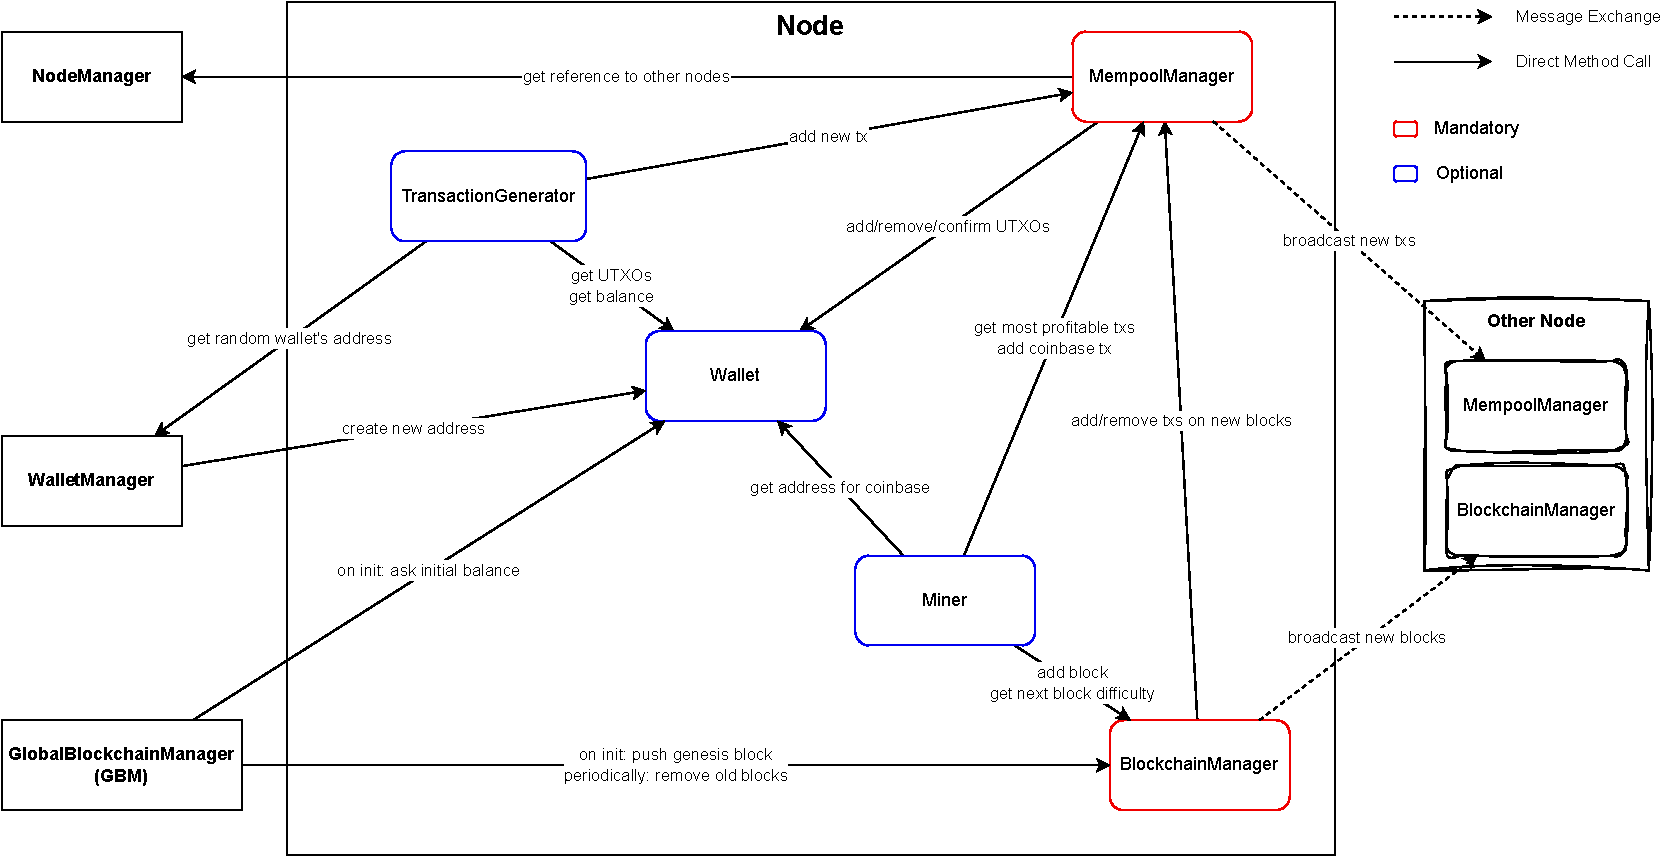
\includegraphics[width=\textwidth]{node-internals}
	\caption{Simple modules (applications) inside a node and the most
	relevant communications between them.}\label{fig:node-internals}
\end{figure}

\subsection{Modular design}\label{subsec:modular-design}

\subsection{Applications}\label{subsec:applications}

This sections describes the applications that are part of a node.
\figref{fig:app-inheritance} shows the inheritance tree of the applications.
The use of the interface \code{IApp} allows to change the implementation of a
specific application only with a configuration change. For example, instead of
the standard \code{BlockchainManager}, a node could use the
\code{SelfishBCManager} described in \secref{sec:selfish-poc} just by inserting
a line in the simulation configuration file:
\begin{verbatim}
Network.node[0].blockchainManager.typename = \
    "iblock.bitcoin.apps.SelfishBCManager"
\end{verbatim}

\begin{figure}[tbhp]
	\centering
	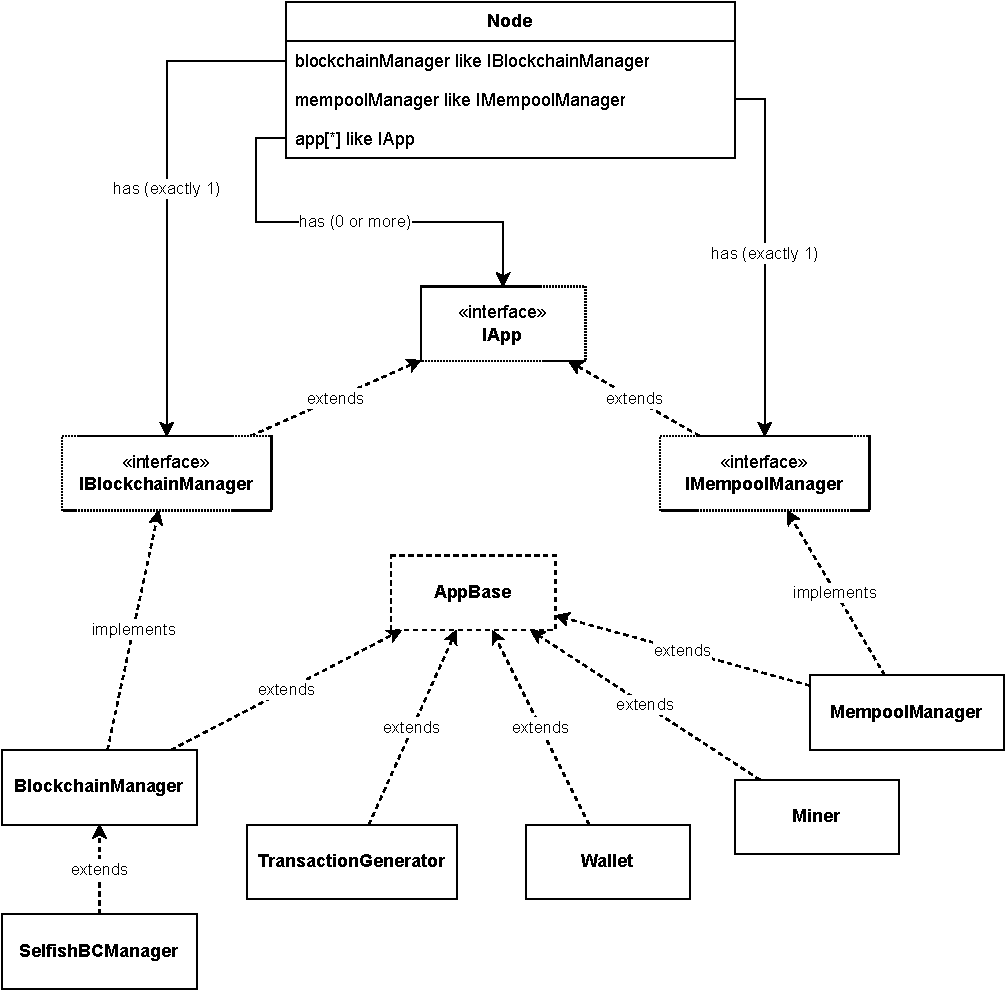
\includegraphics[width=0.8\textwidth]{apps-inheritance}
	\caption{Inheritance tree of the
	applications.}\label{fig:app-inheritance}
\end{figure}

A node can have multiple applications: a miner node, for example, requires a
\code{Miner} application to mine blocks and a \code{Wallet} application to
receive the rewards coming from mining. A node that wants to generate
transactions needs a \code{Wallet} application to store the coins and a
\code{TransactionGenerator} application to generate transactions.

When a message is received from the outside via direct messages (\omnetpp{}'s
\code{sendDirect}), the message is first delivered to the \code{AppBase} class
which in turn calls the \code{handleOtherMessage} method of the application.
The reason behind the name of the method will be discussed later.

The \code{BlockchainManager} and the \code{MempoolManager} applications are
mandatory in any node as they are responsible to maintain the blockchain and
the mempool, respectively.

\subsubsection{BlockchainManager}\label{subsubsec:blockchainmanager}

The \code{BlockchainManager} is responsible for maintaining the blockchain. It
does so by keeping multiple pointer to the head of every branch of the
blockchain. The longest branch is considered the main branch. The developed
application is able to handle forks, chain reorganizations and orphan blocks.

\figref{fig:blockchain-manager-uml} shows the UML diagram of the application.

When a node mines a new block, it broadcasts the block via direct messages to
every other \code{BlockchainManager} in the network. The receiving
\code{BlockchainManager} adds the new block to the blockchain and does the
following:
\begin{enumerate}
	\item If the block is a duplicate block, it is discarded without any
		other side effect;
	\item If the block further extends the main branch it informs the
		\code{MempoolManager} to remove the block's transactions from
		the mempool and the \code{Wallet} application to update the
		number of confirmations associated with each unspent
		transaction output in his possession;
	\item If the block extends a branch that is not the main branch, it
		checks if the branch is longer than the main branch. If so,
		each block in the main branch is removed backward to the
		\emph{fork block} by reinserting the transactions in the
		mempool and unconfirming the UTXOs in the wallet. Then, all
		blocks in the new branch are added to the main branch, one by
		one, by informing the \code{MempoolManager} to remove the
		transactions from the mempool and the \code{Wallet} to confirm
		his UTXOs. If the block is not longer than the main branch, the
		\code{BlockchainManager} just adds the block to the branch;
	\item If the block is an orphan block, it adds it to the array of orphan
		blocks. Orphan blocks are blocks that are received before their
		parent block. When the parent block is received, the orphan
		block is removed from the orphan blocks array and added to the
		blockchain following the same steps as above.
\end{enumerate}

All the above logic is implemented in the \code{appendBlock} method.

At the start of the simulation, the \code{GlobalBlockchainManager} (GBM) module
calls the \code{BlockchainManager}'s \code{addGenesisBlock} to add the genesis
block to the blockchain. The genesis block is a special block which is never
mined in \iblock{}: it is created by the GBM at the start and added to every
\code{BlockchainManager} in the network and it cointains the starting balance
of every \code{Wallet} of the network.

Periodically, the GBM will cal the \code{BlockchainManager}'s \code{cleanup}
method to ask the application to delete the old branches from memory.

When a new block is mined by the local \code{Miner}, it is the responsibility
of the \code{BlockchainManager} to add the block to the blockchain and then
forward the block to the other nodes in the network. This is done by
encapsulating the block in a \code{DirectBlockMsg} message and sending it to
all other nodes via a \code{sendDirect} call. The reference to the other nodes
is obtained from the \code{NodeManager} global module.

Every 2016 blocks, the \code{BlockchainManager} will adjust the difficulty of
the network based on the time needed to mine the last 2016 blocks. This is
implemented in the \code{getNextTargetNBits} method. The difficulty computation
is described in \appendixref{appendix:computations}.

\subsubsection{MempoolManager}\label{subsubsec:mempoolmanager}

The \code{MempoolManager} is responsible for maintaining the mempool. It does
so by a the full list of transactions ordered by their fee rate, thus allowing
an eventual miner to get the list of transactions in the most profitable order.

\figref{fig:mempool-manager-uml} shows the UML diagram of the application.

When a node creates a new transaction, it sends the transaction to every other
\code{MempoolManager} in the network via a direct message. The receiving
\code{MempoolManager} adds the transaction to the mempool and then informs the
wallet if there are new UTxOs that can be spent.

The \code{MempoolManager} class has methods to add and remove transactions from
the mempool. When a transaction is added to the mempool by a local application,
the \code{MempoolManager} contacts the \code{NodeManager} global module to get
the references to all other nodes and then sends the transaction to every other
\code{MempoolManager} by encapsulating it in a \code{DirectTxMsg} message.

\subsubsection{Wallet}\label{subsubsec:wallet}

The \code{Wallet} application is responsible for storing the UTXOs of the node.
Each time the node adds a block to the blockchain or a transaction in the
mempool, the \code{Wallet}'s methods are called to update the list of UTXOs. A
new transaction added to the mempool, causes the \code{MempoolManager} to call
the \code{Wallet}'s \code{addUtxo} method, if the transaction had at least one
output with the \code{Wallet}'s address. When a block is added to the
blockchain, the \code{confirmUtxo} method is used to increase the number of
confirmations of the UTXOs that are still in the wallet. When a transaction
that spends an UTXO is added to the mempool, the \code{removeUtxo} method is
called by the \code{MempoolManager}.

\figref{fig:wallet-uml} shows the UML diagram of the application.

\subsubsection{Miner}\label{subsubsec:miner}

The \code{Miner} application is responsible for mining new blocks. At the start
of the simulation, a \code{nextBlockMsg} timer message is scheduled to be sent
to the \code{Miner} itself. When the message is received, the \code{Miner} will
mine a new block at the top of the current main branch of the blockchain and
inform the \code{BlockchainManager} to add the block to the blockchain (which
will then forward the block to the other nodes in the network). Of course, the
\code{Miner} will also create the coinbase transaction to get the block
reward.

\figref{fig:miner-uml} shows the UML diagram of the application.

Before creating the coinbase transaction, the \code{Miner} asks the
\code{Wallet} application for the address to send the reward. The list of
transactions to include in the block is provided by the \code{MempoolManager}.

The time needed to mine a new block is determined by the \code{Miner}'s hash
rate and the current difficulty of the network. As in the real Bitcoin network,
the difficulty is computed individually by each node and is updated every 2016
blocks by the \code{BlockchainManager}. The computation of the time needed to
mine a block is described in \appendixref{appendix:computations}.

\subsubsection{TransactionGenerator}\label{subsubsec:transactiongenerator}
